
\documentclass[]{article}

\usepackage{dirtytalk}
\usepackage{wrapfig}
\usepackage{listing}
\usepackage{minted}
\usepackage{lipsum}
\usepackage{caption}
\usepackage{braket}
\usepackage{hyperref}
\usepackage{amsmath}
\usepackage{pdflscape}
\usepackage{geometry}
\usepackage{graphicx}
\usepackage{afterpage}
\usepackage{subcaption}
\usepackage[backend=biber]{biblatex}

\bibliography{bibliography}

\hypersetup{colorlinks}

%opening
\title{Fattorizzazione come moltiplicazione \say{Reversed}}
\author{Davide Camino}

\begin{document}
	
	\maketitle
	
	\begin{abstract}
		In questo report vengono presentati alcuni esperimenti sulla fattorizzazione di numeri interi mediante un programma che esegue moltiplicazioni. L'idea consiste nell'implementare in Verilog un programma che moltiplica due valori $A$ e $B$, ottenendo un risultato $C$. Il programma viene quindi trasformato in un circuito digitale e, successivamente, in un problema Ising. La funzione di energia così ottenuta codifica i vincoli logici del circuito, mentre il quantum annealer cerca una configurazione che ne minimizzi l'energia. Il minimo globale corrisponde al soddisfacimento di tutti i vincoli e permette quindi di sfruttare una forma di reversibilità del calcolo: fissando il valore dell'output $C$, le relazioni logiche tra ingressi e uscita consentono di ricavare i fattori $A$ e $B$ come risultato del processo di annealing.
		
		
		Nella Sezione \ref{sec:verilog} viene introdotto il programma Verilog, discutendone le caratteristiche. La Sezione \ref{sec:exp} descrive l'esperimento di fattorizzazione e ne presenta i risultati, mentre nella Sezione \ref{sec:dim} viene analizzata la dimensione del problema Ising in funzione della dimensione del numero da fattorizzare. Infine, nella Sezione \ref{sec:limit} vengono discusse le limitazioni dello studio e proposti alcuni possibili sviluppi futuri.
	\end{abstract}
	
	\section{Programma Verilog}
	\label{sec:verilog}
	
	\begin{wrapfigure}{r}{.55\linewidth}
		\rule{\linewidth}{0.4pt}
		
		\hfill
		\begin{minipage}{.9\linewidth}
			\vspace{.2cm}
			\begin{minted}[linenos=true]{verilog}
module Multiplier (
	input  wire [2:0] A,
	input  wire [2:0] B,
	output wire [5:0] Mul
);

	assign Mul = A * B;

endmodule
			\end{minted}
			\vspace{-.1cm}
		\end{minipage}
		\rule{\linewidth}{0.4pt}
		\captionof{listing}{Multiplier in Verilog}
		\label{lst:mult_verilog}
	\end{wrapfigure}
	
	Un programma Verilog che implementa la moltiplicazione tra due valori può essere descritto a diversi livelli di astrazione. È possibile realizzare un'implementazione che operi a livello di bit, specificando esplicitamente le operazioni da applicare ai singoli bit dei fattori per ottenere il prodotto, oppure sfruttare gli operatori di \say{alto livello} offerti da Verilog, assegnando direttamente a $C$ il risultato della moltiplicazione tra $A$ e $B$. Trattandosi di un'esplorazione preliminare, per questo primo esperimento è stato scelto il secondo approccio. Il codice Verilog che definisce il circuito è riportato nel Listato~\ref{lst:mult_verilog}, la moltiplicazione è definita alla linea 7.
	
	Un altro aspetto importante riguarda il numero di bit assegnati a ciascuna variabile (linee 2--4). Verilog permette di controllare con precisione la dimensione di ogni variabile, caratteristica particolarmente utile per contenere la dimensione del problema Ising finale e studiarne l'andamento al variare delle dimensioni dei dati di ingresso e di uscita. Per dimensionare l'output del circuito si è considerata la relazione:
	\[
	C = A \cdot B,
	\]
	da cui segue:
	\begin{equation}
		\log_2 C = \log_2(A \cdot B) = \log_2 A + \log_2 B.
		\label{eqn:bits}
	\end{equation}
	
	Questa relazione permette di determinare facilmente la dimensione di $C$ a partire da quelle di $A$ e $B$, sebbene presenti alcune limitazioni che verranno discusse in seguito.
	
	\section{Esperimento}
	\label{sec:exp}
	
	Per testare la fattorizzazione è stato scelto di fissare $C = 35$. Questo è il valore più grande rappresentabile su $6$ bit che sia il prodotto di due numeri primi scrivibili su 3 bit e non sia un quadrato perfetto. Fissato il valore di $C$, ci si aspetta che la coppia $\braket{A, B}$ valga $\braket{5, 7}$ oppure $\braket{7, 5}$.
	
	\subsection{Set Sperimentale}
	
	Il problema in forma Ising è stato ottenuto utilizzando la pipeline presentata nel report precedente \cite{Camino_Sperimentando}. Per la sintesi dei circuiti logici sono stati impiegati diversi insiemi di porte, ottenendo circuiti con un numero differente di gates e problemi Ising con un diverso numero di qubit:
	
	\begin{enumerate}
		\label{enum:set}
		\item $\set{\texttt{AND}, \texttt{NOT}}$: 68 gates, 68 qubit;
		\item $\set{\texttt{AND}, \texttt{OR}, \texttt{NOT}}$: 61 gates, 61 qubit;
		\item $\set{\texttt{AND}, \texttt{OR}, \texttt{NAND}, \texttt{NOR}, \texttt{NOT}}$: 38 gates, 38 qubit;
		\item $\set{\texttt{AND}, \texttt{OR}, \texttt{NAND}, \texttt{NOR}, \texttt{XOR}, \texttt{NOT}}$: 30 gates, 38 qubit (per ogni porta \texttt{XOR} è necessario un qubit ancilla).
	\end{enumerate}
	
	Per costruire il problema Ising, a ciascuna porta logica è stata associata una funzione pseudobooleana che richiedesse il minor numero possibile di variabili ancilla\footnote{Le definizioni delle funzioni pseudobooleane, rappresentate mediante matrici triangolari superiori, sono disponibili all'indirizzo \url{https://github.com/DavideCamino/Reports/blob/main/Gates_to_Ising/code/utility/gate_penalties.json}}. Questa scelta deriva dai risultati ottenuti in precedenza, che hanno mostrato come la qualità delle soluzioni migliori al diminuire della dimensione del problema, ovvero del numero di qubit utilizzati \cite{Camino_Sperimentando}.
	
	Per risolvere i problemi in forma Ising è stata uasta la libreria OpenQUOPS\footnote{\url{https://github.com/DavideCamino/OpenQUOPS}} che mette a disposizione Simulated Annealing (SA) e Simulated Quantum Annealing (SQA) attraverso il framework Ocean di D-Wave\footnote{\url{https://docs.dwavequantum.com/en/latest/ocean/}}. Per ottenere risultati statisticamente significativi, ciascun problema è stato risolto $30$ volte con entrambi i metodi, raccogliendo per ogni esecuzione $2^{16} \approx 65\,000$ campioni. Ogni campione rappresenta un assegnamento dei valori di $A$ e $B$. Al termine delle $30$ esecuzioni, per ciascun assegnamento distinto di $A$ e $B$ sono state calcolate la media e la deviazione standard del numero di osservazioni.
	
	Non sono stati condotti esperimenti con QAOA, poiché la simulazione dell'algoritmo avrebbe richiesto una quantità eccessiva di memoria; OpenQUOPS, infatti, implementa QAOA grazie a Qiskit e Qiskit Aer. Attualmente, il metodo di simulazione impiegato da \texttt{AerSimulator} è \texttt{statevector}, il cui costo in termini di memoria è $O(2^n)$, dove $n$ rappresenta il numero di qubit \cite{qiskit_aer_aersimulator}. Questo costo rende impraticabile la simulazione di circuiti con un numero così elevato di qubit come quelli presentati nell'Elenco \ref{enum:set}.
	
	Tutto il codice necessario per eseguire gli eperimenti è disponibile nello stesso repository del report\footnote{\url{https://github.com/DavideCamino/Reports/tree/main/Factorization}}
	
	\subsection{Risultati}
	
	I risultati ottenuti sono riportati nella Figura \ref{fig:fact}. Si osserva che SA produce soluzioni di qualità superiore rispetto a SQA, sebbene entrambi i metodi mostrino un comportamento complessivamente simile. Le distribuzioni degli assegnamenti presentano infatti forme confrontabili, ma le soluzioni ottenute con SQA risultano più rumorose. Questo suggerisce che entrambi i metodi tendano a rimanere intrappolati negli stessi minimi locali, con una frequenza maggiore nel caso di SQA.
	
	Si osserva inoltre che, indipendentemente dal metodo di risoluzione utilizzato, la qualità dei risultati migliora al diminuire del numero di qubit. Confrontando le soluzioni ottenute dai circuiti sintetizzati con gli insiemi di porte $3$ e $4$ dell'elenco \ref{enum:set}, emerge che, a parità di qubit, il circuito con un numero maggiore di gates produce risultati migliori. Questo comportamento merita un'analisi più approfondita. Per il momento, si può ipotizzare che un numero maggiore di gates corrisponda a un circuito classico più profondo e, di conseguenza, a una matrice più sparsa. Una funzione di energia con queste caratteristiche potrebbe risultare più semplice da minimizzare.
	
	
	
	\section{Analisi della dimensione del problema Ising}
	\label{sec:dim}
	
	\begin{wrapfigure}[18]{r}{.57\linewidth}
		\centering
		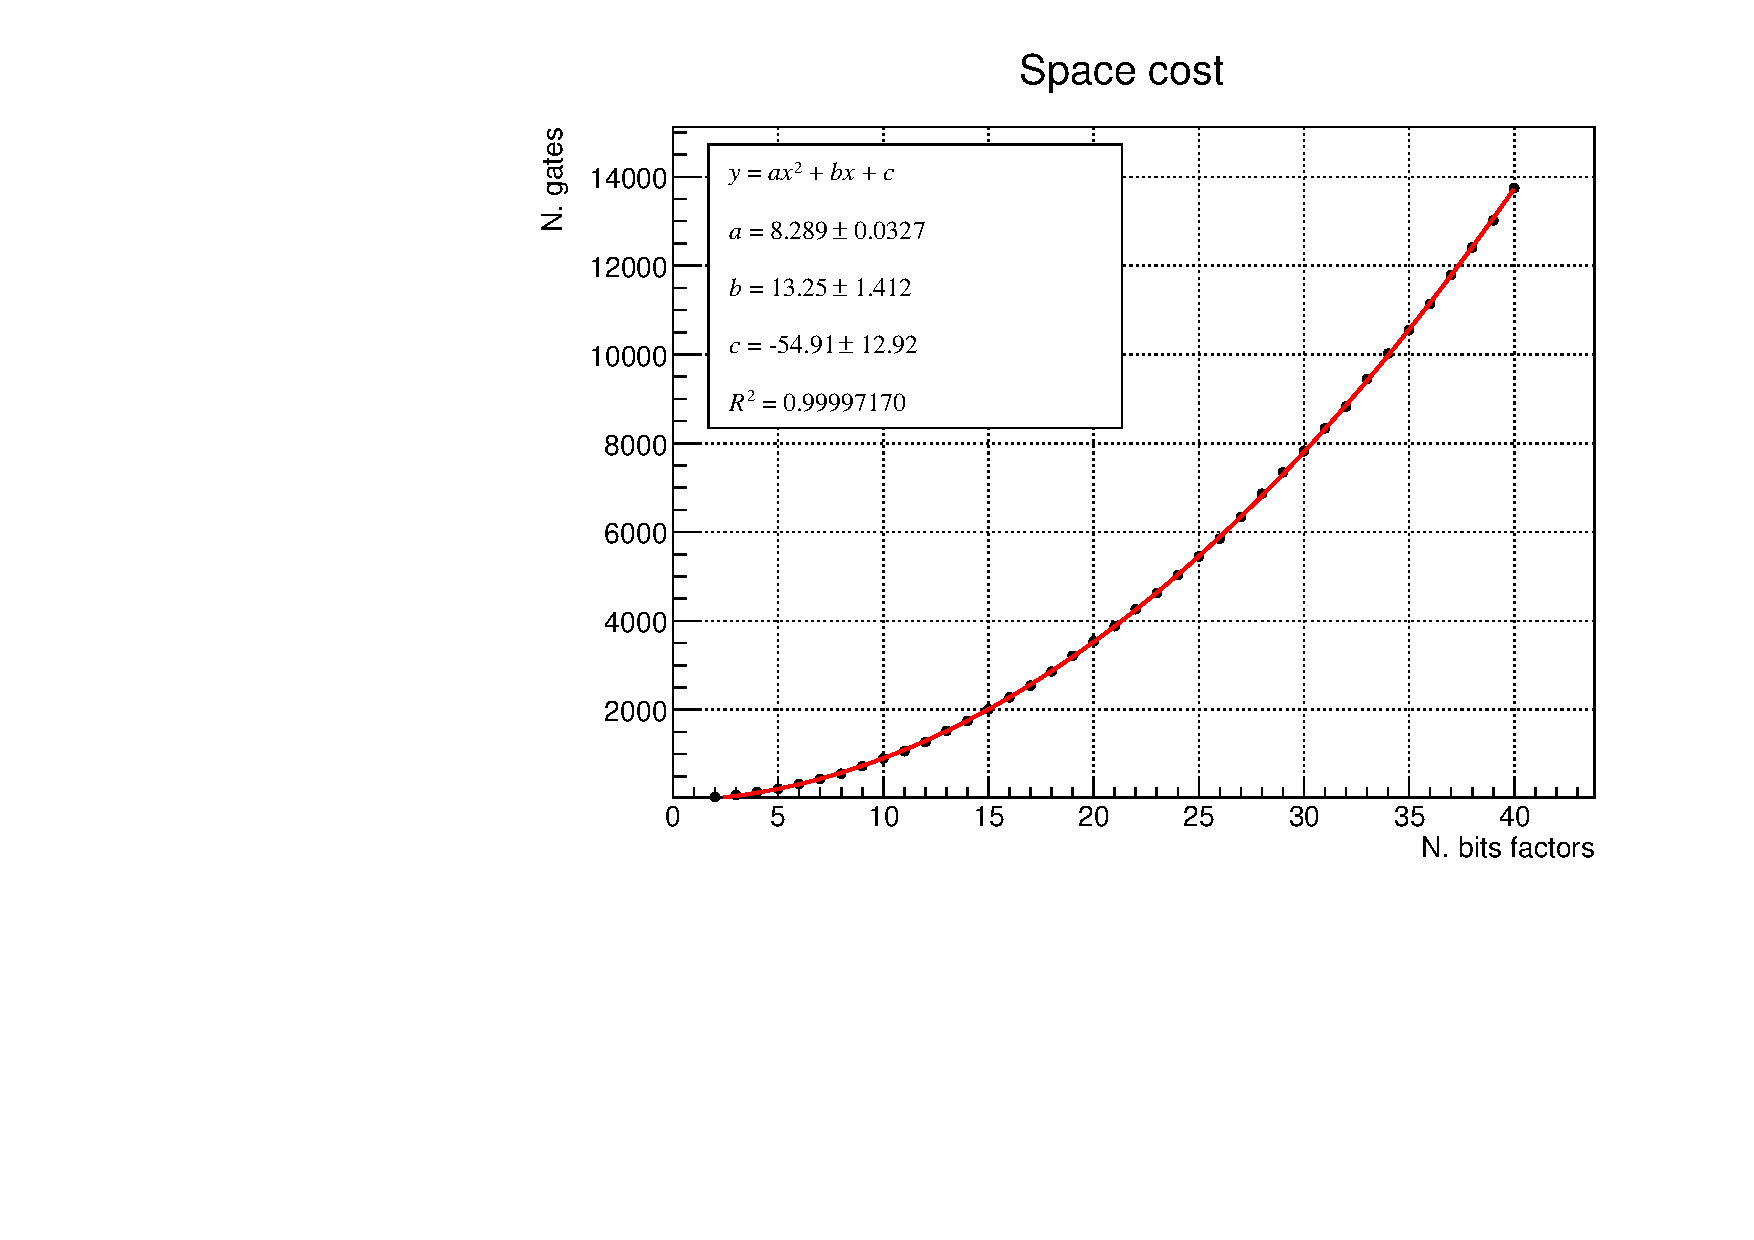
\includegraphics[width=\linewidth]{Pictures/dim}
		\caption{Gates in funzione dei bits dei fattori $A$ e $B$}
		\label{fig:dim}
	\end{wrapfigure}
	Per analizzare la crescita della dimensione del problema Ising in funzione della dimensione dei fattori, è necessario esaminare preliminarmente come varia la dimensione del circuito sintetizzato. In questa prima analisi non vengono considerati gli aspetti propri dell'ingegneria elettronica, ma ci si limita a studiare i circuiti prodotti attraverso Yosys.
	
	
	
	In particolare, partendo dal codice riportato nel Listato \ref{lst:mult_verilog}, utilizzandolo come \say{template} e considerando la Formula \ref{eqn:bits} per dimensionare il risultato, vengono generati circuiti in grado di accettare in ingresso numeri progressivamente più grandi. La Figura \ref{fig:dim} mostra l'andamento del numero di gates in funzione del numero di bit assegnati a ciascun fattore della moltiplicazione. Il valore di $R^2$, molto vicino a $1$, suggerisce che il modello di crescita quadratica ipotizzato descriva adeguatamente l'aumento del numero di gates del circuito.
	
	Poiché ogni gate contribuisce con un numero costante di qubit alla rappresentazione del problema Ising, anche la dimensione del problema finale cresce quadraticamente rispetto alla dimensione dell'input.
	
	Questo è un risultato importante perché mostra che la trasformazione del problema di fattorizzazione in un problema Ising non introduce una crescita esponenziale nel numero di variabili necessarie a rappresentarlo. Se la dimensione del circuito crescesse esponenzialmente rispetto a quella dell'input, la sola rappresentazione del problema richiederebbe risorse esponenziali, rendendo questo approccio difficilmente praticabile. La crescita quadratica osservata evita questa limitazione, anche se non garantisce che il problema Ising risultante possa essere risolto efficientemente: il costo computazionale necessario a individuare il minimo globale della funzione di energia potrebbe comunque crescere esponenzialmente.
	
	\subsection{E Shor?}
	
	Il lavoro più recente che è stato individuato e si concentra sul numero di qubit logici necessari per implementare l'algoritmo di Shor risale al 2024 \cite{chevignard2025reducing}. Indicando con $N$ il numero da fattorizzare e ponendo $n = \log_2 N$, il numero di qubit richiesti per implementare l'algoritmo di Shor è pari a $\frac{n}{2} + o(n)$. Il numero di gates è dell'ordine di $O(n^3)$, mentre la profondità del circuito è pari a $n^2 \log^3 n$. Inoltre, il circuito deve essere eseguito più volte. L'articolo stima, ad esempio, che per fattorizzare una chiave RSA a $2048$ bit siano necessari $1730$ qubit logici e $40$ esecuzioni del circuito.
	
	Questo risultato è interessante perché, nonostante il numero di qubit logici richiesto dall'algoritmo di Shor sia inferiore, la dimensione del circuito quantistico da realizzare cresce più rapidamente rispetto a quella del problema Ising. Questo comporta anche un maggior numero di errori introdotti durante l'esecuzione e la necessità di utilizzare più qubit fisici per compensare la scarsa affidabilità dei gates quantistici. Ciò non implica che l'approccio proposto sia più efficiente dell'algoritmo di Shor, ma suggerisce che non debba essere escluso a priori per il solo fatto che il numero di qubit richiesti cresce quadraticamente.
	
	\section{Limitazioni e spunti}
	\label{sec:limit}
	
	Un primo aspetto da approfondire riguarda la progettazione dei circuiti moltiplicatori. Sarebbe utile acquisire maggiori conoscenze di elettronica digitale per comprendere come descrivere direttamente un moltiplicatore. Yosys produce risultati soddisfacenti, ma il tempo richiesto per l'ottimizzazione diventa considerevole quando il numero di gates cresce. La struttura di un moltiplicatore presenta certamente delle regolarità e, una volta compreso come assemblare le porte logiche, non sembra irragionevole ipotizzare che la sintesi di un circuito la cui dimensione cresce quadraticamente con quella dell'input possa essere eseguita anch'essa in tempo quadratico.
	

	Un'altra limitazione riguarda l'impossibilità di testare QAOA a causa dell'elevato consumo di memoria. Esistono tuttavia metodi di simulazione alternativi a \texttt{statevector}, tra cui \texttt{stabilizer}, \texttt{extended\_stabilizer} e \texttt{matrix\_product\_state} \cite{qiskit_aer_aersimulator}. I primi due sono adatti principalmente a circuiti costruiti con porte di Clifford o con un numero limitato di porte non-Clifford. Il terzo è particolarmente interessante perché permette di rappresentare lo stato quantistico in forma compatta, purché il grado di entanglement non sia troppo elevato. Per valutarne l'applicabilità sarà quindi necessario studiare l'entanglement generato da QAOA. Inoltre, sarà necessario aggiornare OpenQUOPS per supportare metodi di simulazione alternativi a \texttt{statevector}.

	
	Un'ulteriore limitazione riguarda il dimensionamento delle variabili di ingresso e di uscita. La scelta adottata funziona correttamente quando si parte dalle dimensioni dei fattori per determinare quella del prodotto, ma risulta meno efficace nel caso inverso. Considerando nuovamente il Listato \ref{lst:mult_verilog}, l'output permette di rappresentare valori fino a $63$, mentre il valore più grande che può essere espresso come prodotto di due numeri primi rappresentabili su $3$ bit è $49 = 7 \cdot 7$. Si consideri tuttavia un numero più piccolo, ad esempio $26$. Poiché $26 < 49$, ci si potrebbe aspettare che la sua fattorizzazione non presenti problemi. In realtà, essendo $26 = 2 \cdot 13$, non è possibile rappresentare entrambi i fattori utilizzando soltanto $3$ bit per ciascuno. Sarebbe quindi opportuno approfondire il criterio con cui vengono dimensionati gli ingressi e l'uscita del circuito. Va comunque osservato che, nel caso di RSA, i due fattori hanno tipicamente ordini di grandezza simili, per cui è improbabile incontrare situazioni in cui uno dei numeri primi sia molto piccolo rispetto all'altro.
	
	\printbibliography
	
	
\afterpage{%
	\clearpage
	\newgeometry{margin=0.5cm}
	\begin{landscape}
		%\thispagestyle{empty}
		\begin{figure}[h]
			\begin{subfigure}{.49\linewidth}
				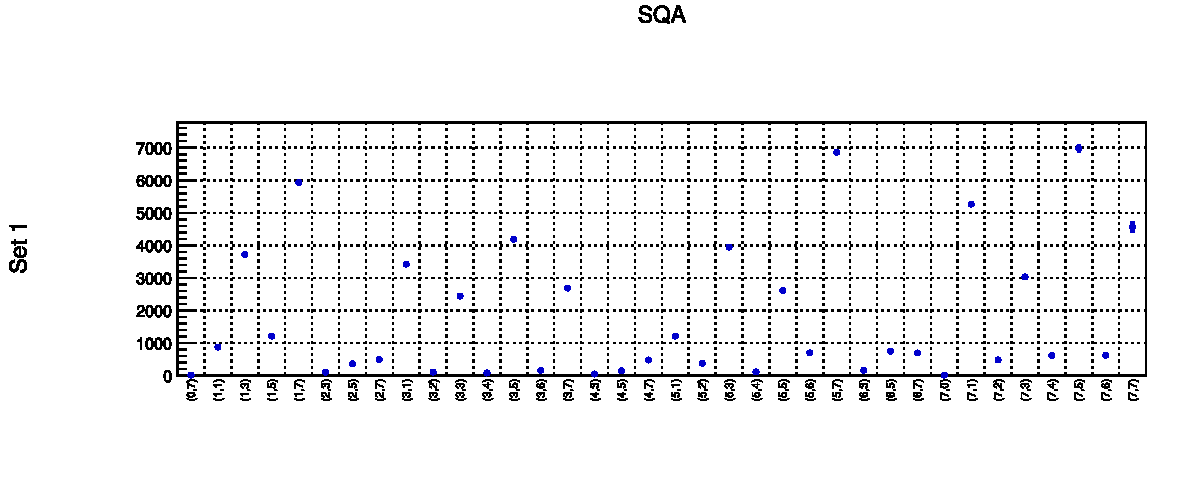
\includegraphics[width=1.08\linewidth]{Pictures/1}
			\end{subfigure}
			\hspace{-.73cm}
			\begin{subfigure}{.49\linewidth}
				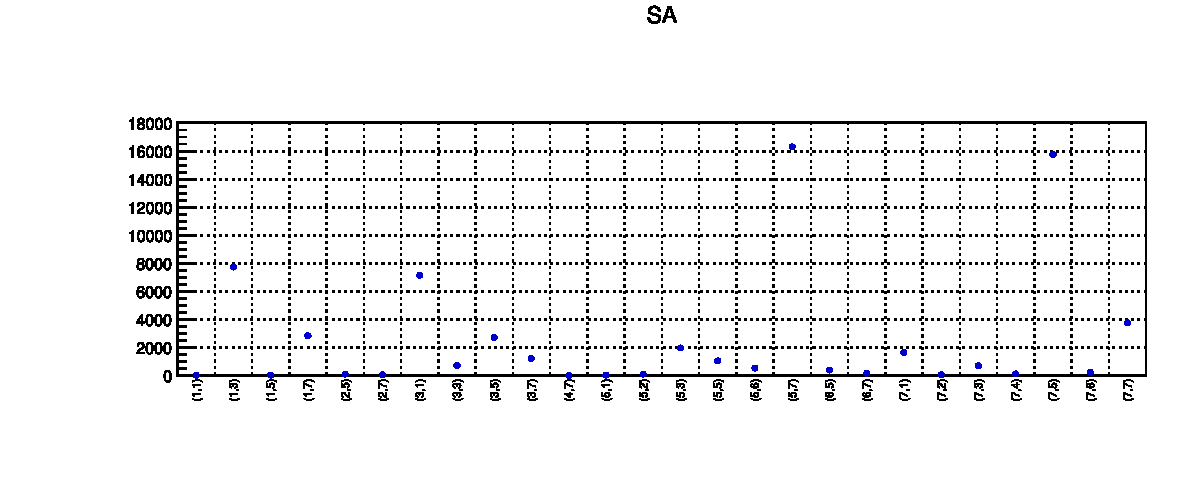
\includegraphics[width=1.08\linewidth]{Pictures/2}
			\end{subfigure}
			
			\vspace{-1.8cm}
			\begin{subfigure}{.49\linewidth}
				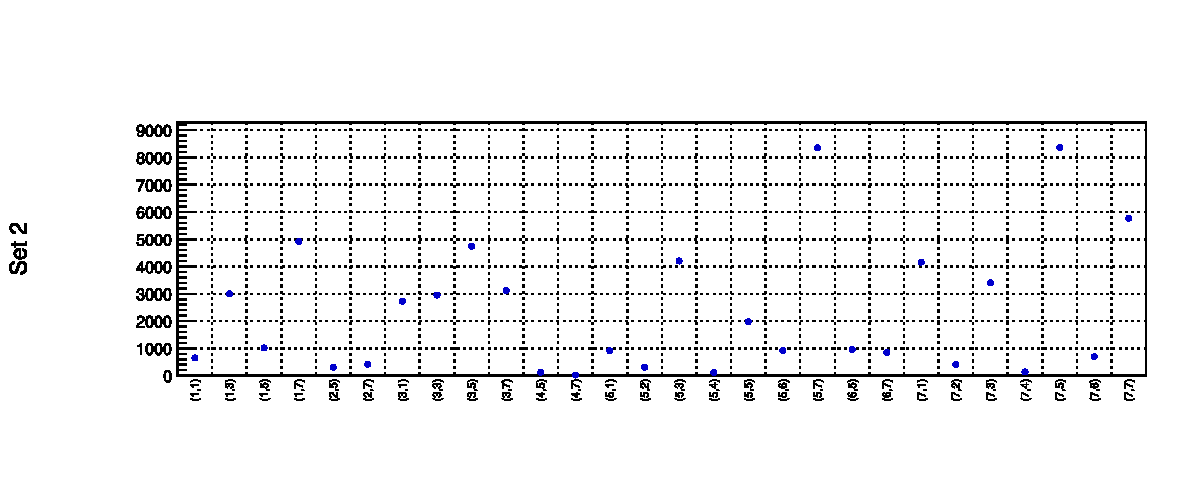
\includegraphics[width=1.08\linewidth]{Pictures/3}
			\end{subfigure}
			\hspace{-.73cm}
			\begin{subfigure}{.49\linewidth}
				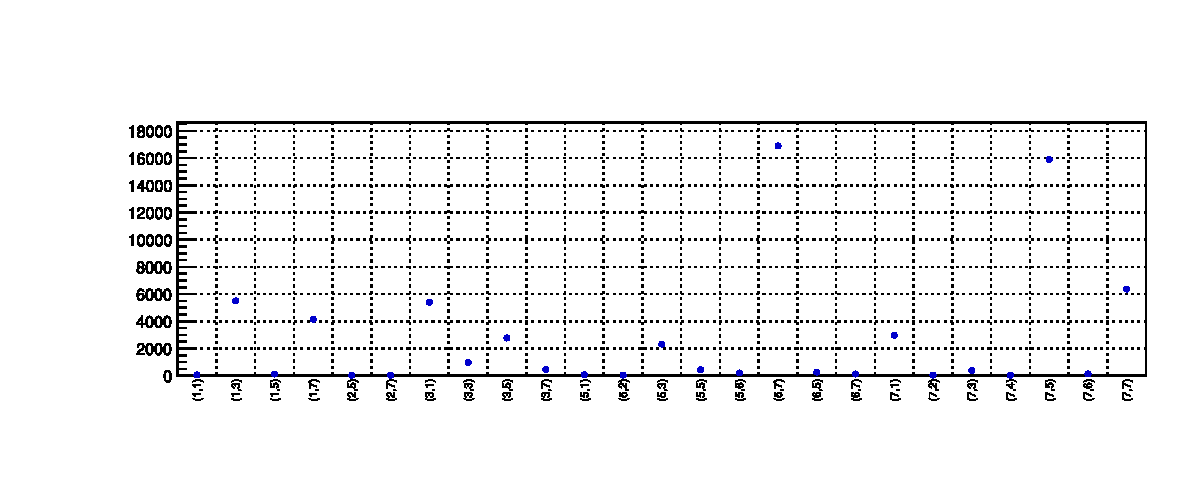
\includegraphics[width=1.08\linewidth]{Pictures/4}
			\end{subfigure}
			
			\vspace{-1.8cm}
			\begin{subfigure}{.49\linewidth}
				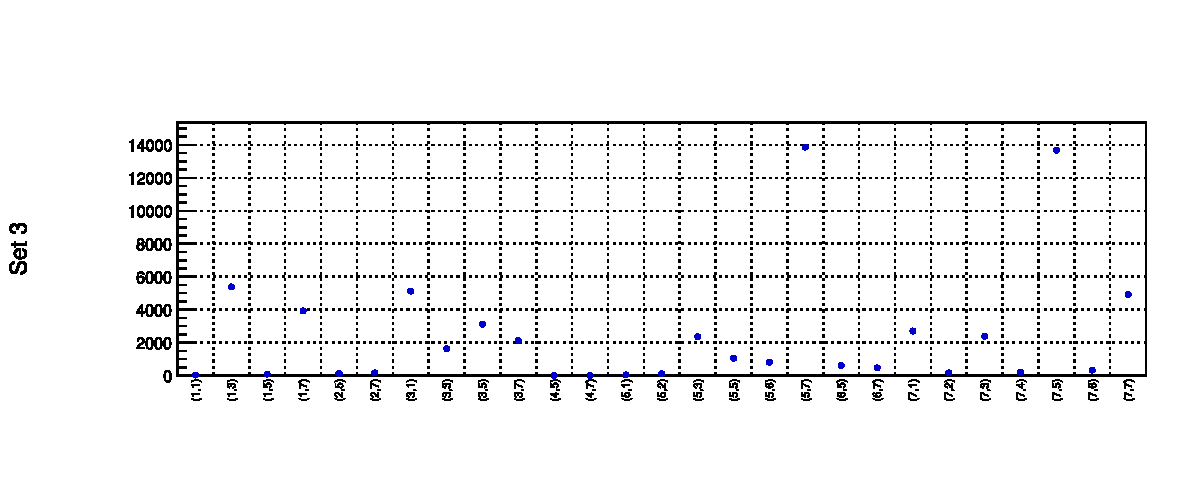
\includegraphics[width=1.08\linewidth]{Pictures/5}
			\end{subfigure}
			\hspace{-.73cm}
			\begin{subfigure}{.49\linewidth}
				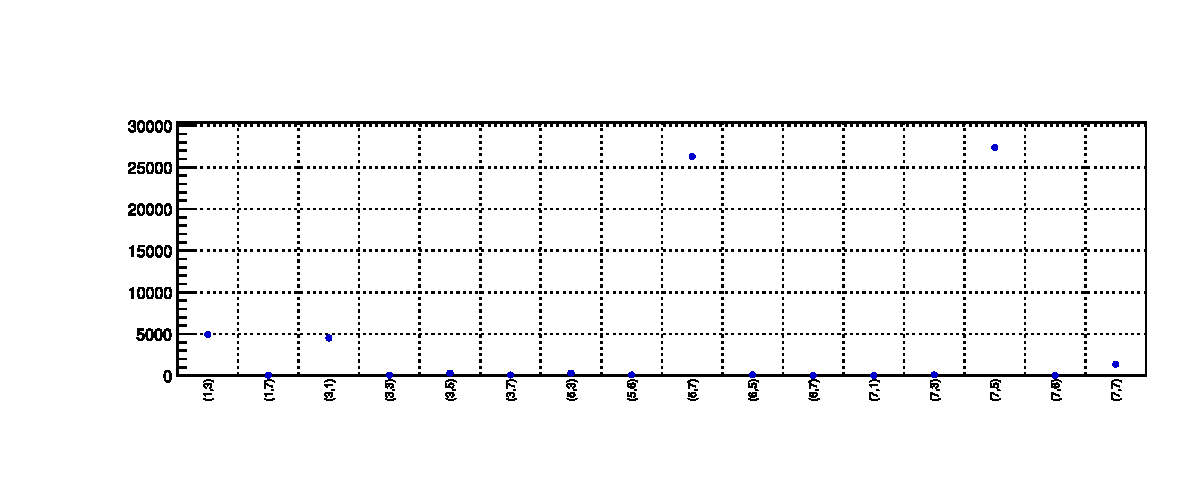
\includegraphics[width=1.08\linewidth]{Pictures/6}
			\end{subfigure}
			
			\vspace{-1.8cm}
			\begin{subfigure}{.49\linewidth}
				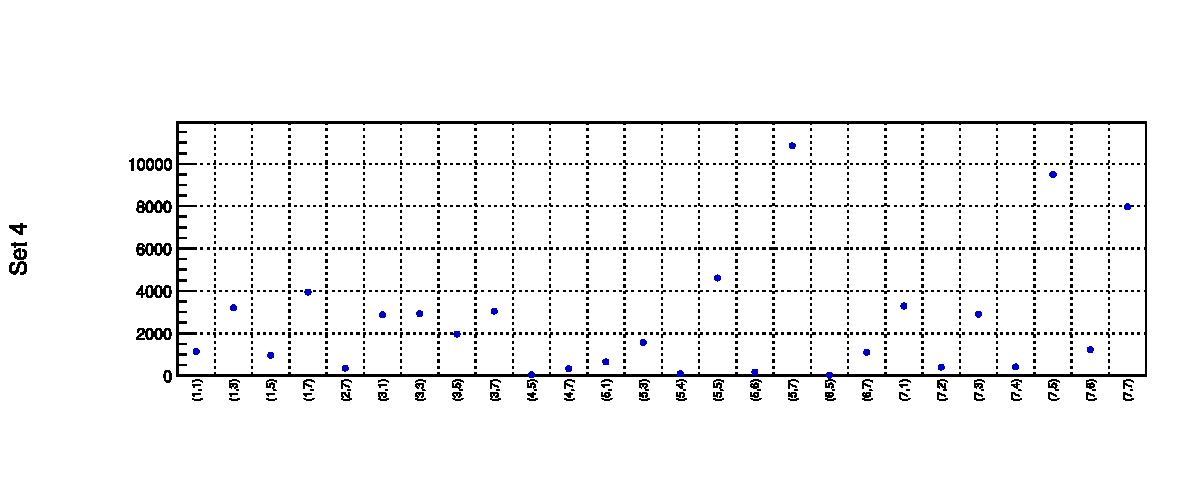
\includegraphics[width=1.08\linewidth]{Pictures/7}
			\end{subfigure}
			\hspace{-.73cm}
			\begin{subfigure}{.49\linewidth}
				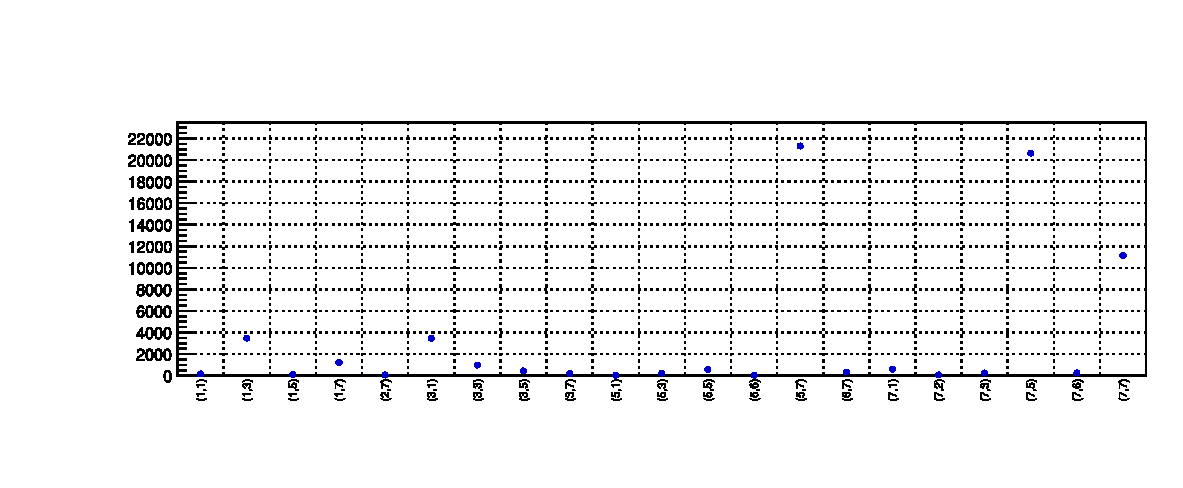
\includegraphics[width=1.08\linewidth]{Pictures/8}
			\end{subfigure}
			\caption{La Figura si legge come una tabella, sulle righe ci sono i diversi set di porte utilizzate (con riferimento all'Elenco \ref{enum:set}), sulle colonne i diversi metodi di risoluzione; sull'asse $x$ di ogni grafico leggiamo gli assegnamenti di $A$ e $B$ osservati; sull'asse $y$ il numero medio di osservazioni per un certo assegnamento, l'errore associato alla misura è la deviazione standard.}
			\label{fig:fact}
		\end{figure}
	\end{landscape}
	\restoregeometry
}

	
\end{document}
